%TODO: refer to grid convolutions as discrete (?)


\chapter{Introduction}
\label{chap:intro}

Many cellular processes rely on proteins, which facilitate these processes via their interactions with one another and with small molecules within the cell~\cite{scheeffink2003}.
%TODO: mention protein interaction networks?
A more complete understanding of how proteins interact with one another can provide insight into many diseases, aid pharmaceutical research~\cite{fauman2003}, and improve our understanding of complex cellular processes~\cite{altman2003}.
Proteins normally interact with one another via an \textit{interface}, which is comprised of amino acid residues in each protein which participate in the interaction.

Experimentally identifying the interface between two proteins is a time consuming and expensive process which involves crystallization of the protein complex, and imaging via x-ray crystallography or nuclear magnetic resonance~\cite{bijelic2017}\cite{ilarisavino2017}\cite{wang2017}.
In contrast, \textit{in silico} methods are faster and cheaper, and may detect unforeseen interfaces to help inform the potential relevance of various wet lab experiments.
Various such methods exist, some predicting whether a single amino acid residue is a part of any interface~\cite{}, others predicting whether a pair of amino acid residues from different proteins constitutes part of the interface between them~\cite{ahmad2011}\cite{minhas2014}.
In addition, some related approaches first predict the bound 3D structure of the protein complex, from which the interface can be extracted~\cite{chen2003}\cite{dominguez2003}.

This thesis presents a novel method of predicting which amino acid pairs are part of an interface, which is inspired by the success of convolutional neural networks in image processing~\cite{gu2015}\cite{lecun2010}.
Proteins are represented as graphs and fed into a pairwise convolutional neural network with specialized convolution operations.
The network makes predictions on pairs of amino acids of the likelihood that they constitute a part of the interface. 
This method outperforms the existing state-of-the-art approach based on a support vector machine with pairwise kernels~\cite{minhas2014}.
The remainder of the introduction presents a primer on proteins and their interfaces. 

The rest of this thesis is organized as follows.
%TODO: Update when done
Chapter \ref{chap:methods} describes the graph convolutional networks and the deep learning architecture I used for interface prediction.
Chapter \ref{chap:experiments} describes the data set and experiments performed and presents findings. 
Chapter \ref{chap:future} lays out potential avenues of research which build upon the findings in this thesis. 
Appendix \ref{appendix:features} contains details pertaining to the features computed for each amino acid residue, and Appendix \ref{appendix:tools} describes the software and tools that were created and/or used for this research.

\section{Proteins}

DNA is often considered the "blueprint for life." 
In that case, proteins are the physical realization of those blueprints.
In other words, the information contained in DNA is ultimately used to synthesize proteins.
Proteins are composed of amino acids linked in a chain and held together by covalent bonds.
Amino acids are organic compounds consisting of a central \textit{$\alpha$-carbon} atom, which binds to an \textit{amine group} ($NH_2$), a \textit{carboxyl group} ($COOH$), a single hydrogen atom, and a \textit{side chain}, in a tetrahedral geometry.
There are 20 different types of amino acid, each of which has a different side chain that gives rise to distinct structural and electro-chemical properties.
Figure \ref{fig:aminoacids} depicts the different types of amino acids, borrowed from~\cite{scheeffink2003}.

%TODO: copyright issues with  these figures?

\begin{figure}
	\centering
	%\begin{center}
	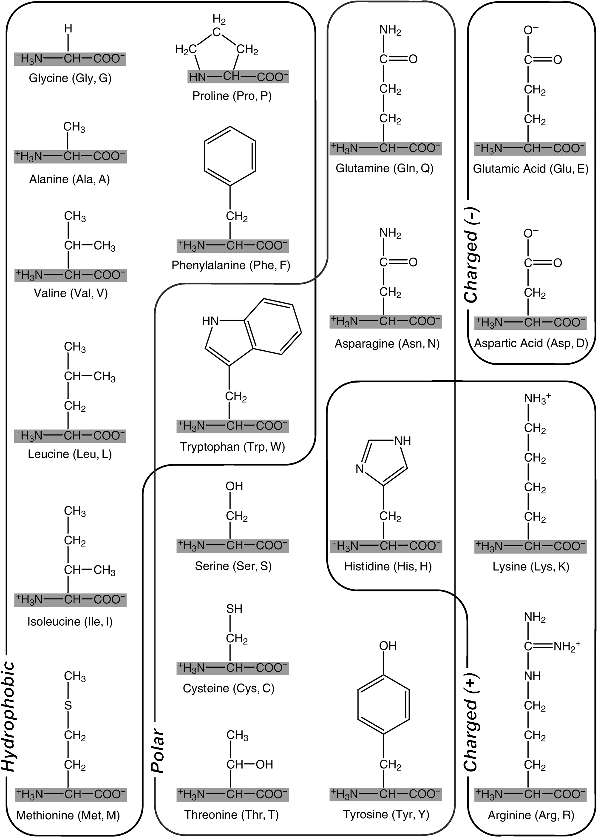
\includegraphics[width=0.8\textwidth]{wiley_liss_structural_bioinformatics_amino_acids.png}
	%\end{center}
	\caption{The 20 types of amino acid, each with a distinct side chain. In this figure, the carboxyl group has lost a hydrogen leaving a negative charge, and the amine group has gained a hydrogen leaving a positive charge. The elements which make up a peptide backbone are highlighted in gray, in addition to the hydrogen which connects to the $\alpha$-carbon. The side chains give rise to various electrical properties, as indicated by the circumscriptions. Taken from~\cite{scheeffink2003}.}
	\label{fig:aminoacids}
\end{figure}

Amino acids link together when the nitrogen atom from one protein's amine group bonds covalently with the carbon atom of another protein's carboxyl group, releasing a water molecule in the process.
This covalent bond is called a peptide bond, and an amino acid involved in at least one such bond is referred to as an \textit{amino acid residue}, or \textit{residue}.

A \textit{peptide}, or \textit{peptide chain}, is a linear chain of amino acids held together by peptide bonds, and the \textit{backbone} of the peptide consists of all atoms participating in peptide bonds together with the $\alpha$-carbons.
If a peptide contains several residues it is referred to as a \textit{polypeptide}.
Proteins consist of one or more polypeptides which are bound together.
All peptides have a natural ordering of their amino acid residues defined by the order in which they were incorporated into the peptide during protein synthesis.
The first residue to be incorporated has a free amine group denoted the \textit{N-terminus}, whereas the last residue has a free carboxyl group denoted the \textit{C-terminus}.
Figure \ref{fig:3res} shows a model of three adjacent residues from a larger polypeptide.

\begin{figure}
	\centering
	%\begin{center}
	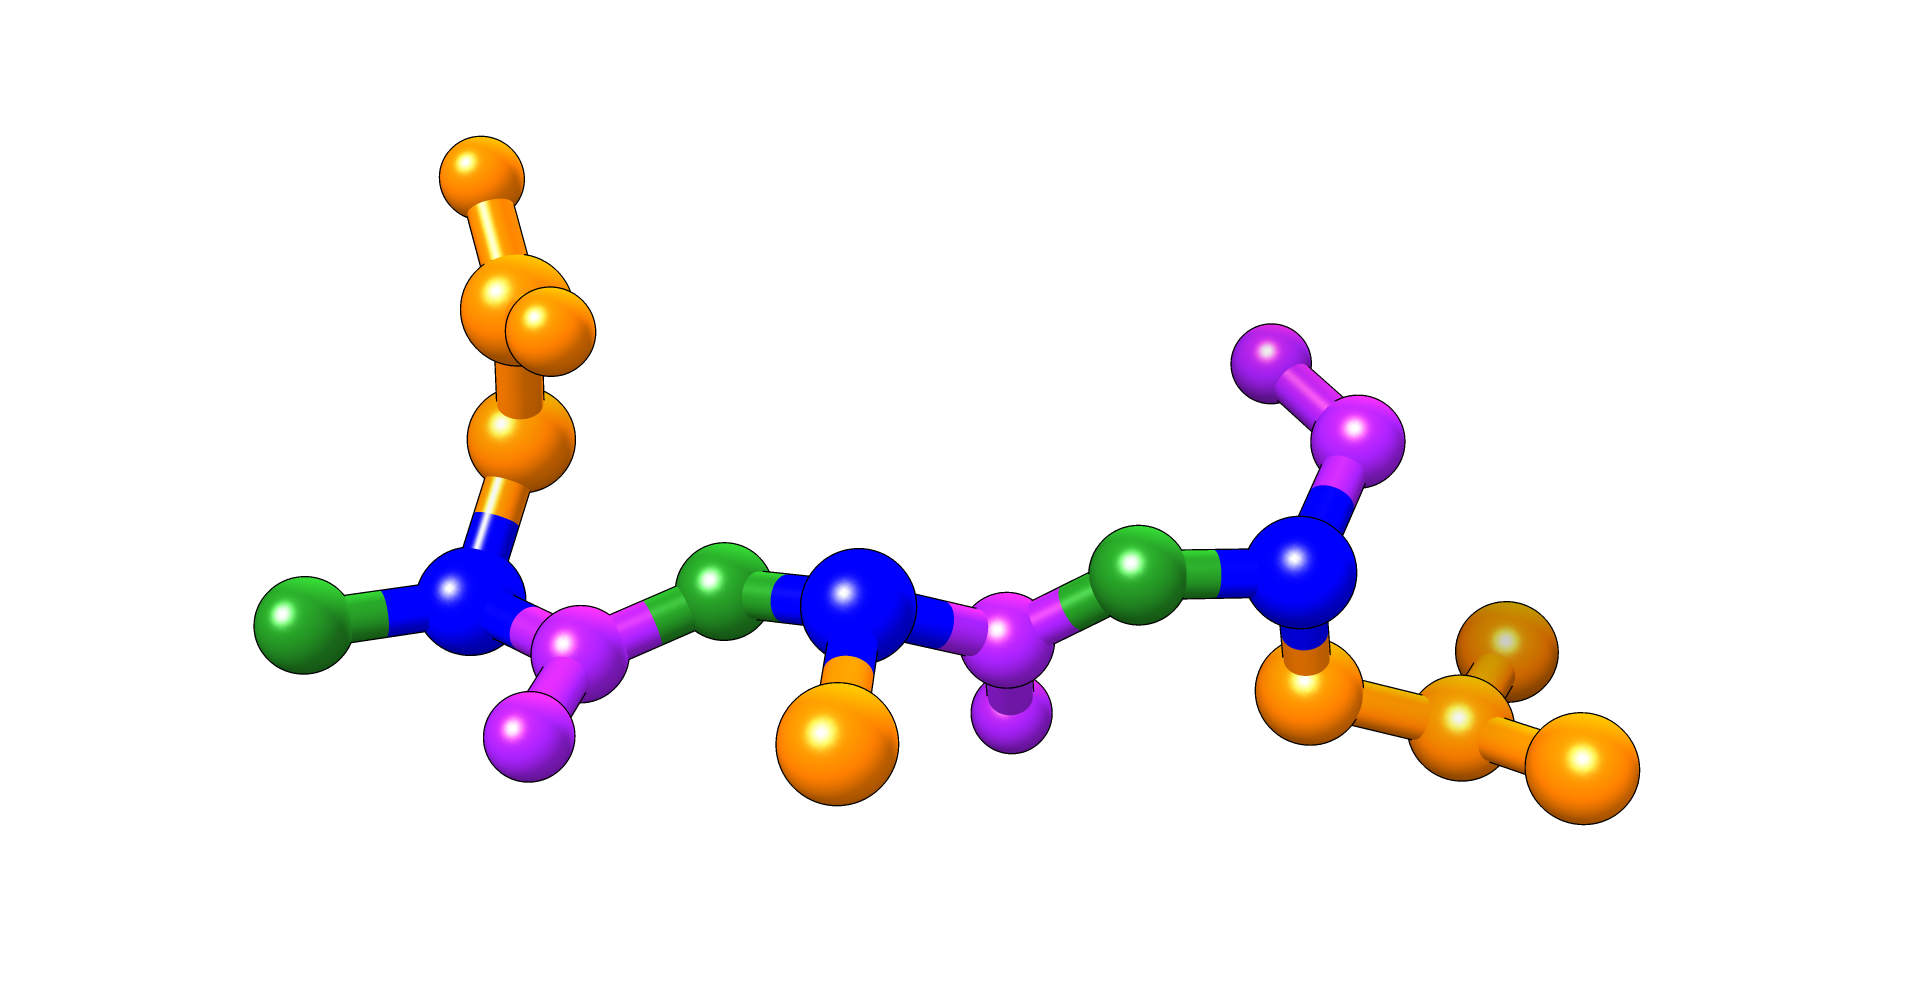
\includegraphics[width=0.8\textwidth]{1dab_3res_3x3.png}
	%\end{center}
	\caption{Ball and stick model of a three amino acid residue section from a larger polypeptide (hydogens omitted). Colors indicate, blue: $\alpha$-carbon , orange: side chain, purple: carboxyl group after loss of OH, green: amine group after loss of H. Peptide bonds are between purple and green atoms. The backbone extends horizontally along blue, purple, and green atoms. Each sequence of atoms starting at an $\alpha$-carbon and ending at the next $\alpha$-carbon lay in an amide plane. From left to right are Aspartic Acid, Alanine, and Leucine. Created with Chimera~\cite{pettersen2004}.}
	\label{fig:3res}
\end{figure}

A residue's side chain can influence how it interacts with other amino acids or other atoms and molecules. For example, oppositely charged side chains will be attracted to each other, and polar and non-polar side chains will not strongly interact with each other. 
Polar side chains are also called hydrophilic due to their affinity for water, and non-polar side chains are also called hydrophobic for the opposite reason.
Such interactions play an important role in how proteins fold into 3D structures \cite{scheeffink2003}.

%TODO: mention globular proteins vs other kinds?


\subsection{Protein Structure}

Protein structure can be described via four levels of abstraction. 
\textit{Primary structure} refers to the sequence of amino acid residues (from N-terminus to C-terminus) in a single polypeptide, and is determined by the sequence of codons in the corresponding coding mRNA from which the protein is translated.
Sequences are typically written using a string of letters, where each unique letter corresponds to a different residue type. 

The physical chemistry associated with peptide bonds gives rise to the property that the nitrogen and carbon atoms involved in the peptide bond, along with the adjacent $\alpha$-carbons, all lie within a plane, called the \textit{amide plane}.
Each $\alpha$-carbon lies on the intersection between two amide planes, and the planes are free to rotate with respect to each other. 
%TODO: figure?
In some cases, side chains prohibit certain relative angles due to \textit{steric constraints}, which enforce that no two atoms may occupy the same volume of space at the same time.
The angle between amide planes allows a certain amount of flexibility in the peptide backbone, which gives rise to higher order structures.

\textit{Secondary structure} describes the local structures that arise from the interaction of non-adjacent residues in a polypeptide.
There are three common categories of local structures: $\alpha$-helices, $\beta$-sheets, and loops.
An  $\alpha$-helix occurs when the polypeptide coils into a barrel-like structure (like the threads of a screw) and residues from adjacent coils (a distance of three residues from each other along the backbone) form hydrogen bonds with one another.
A $\beta$-sheet occurs when two non-adjacent sections of the polypeptide align next to each other such that residues in one of the sections form hydrogen bonds with residues in the other section.
$\beta$-sheets may be parallel or anti-parallel, depending on the relative orientation of adjacent strands in the sheet.
Figure \ref{fig:beta} illustrates the difference between parallel and anti-parallel $\beta$-sheets.
\begin{figure}
	\centering
	%\begin{center}
	\subfloat[Parallel $\beta$-sheets]{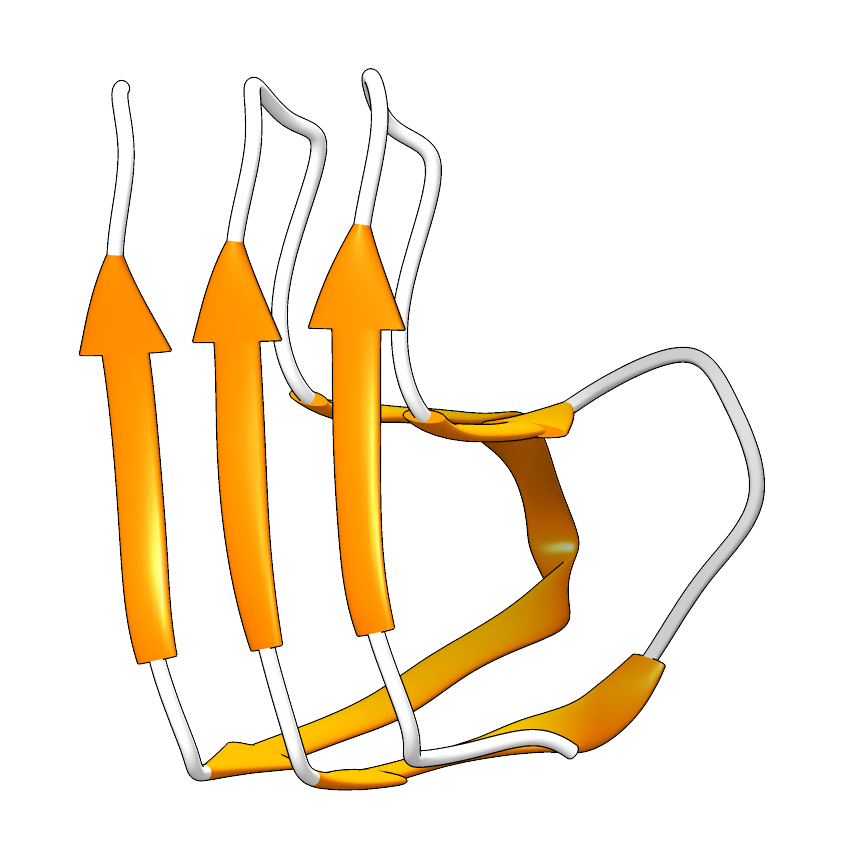
\includegraphics[width=0.4\textwidth]{1dab_end_betaP_3x3_cropped.png}\label{fig:beta_para}}
	\hfill
	\subfloat[Anti-parallel $\beta$-sheets]{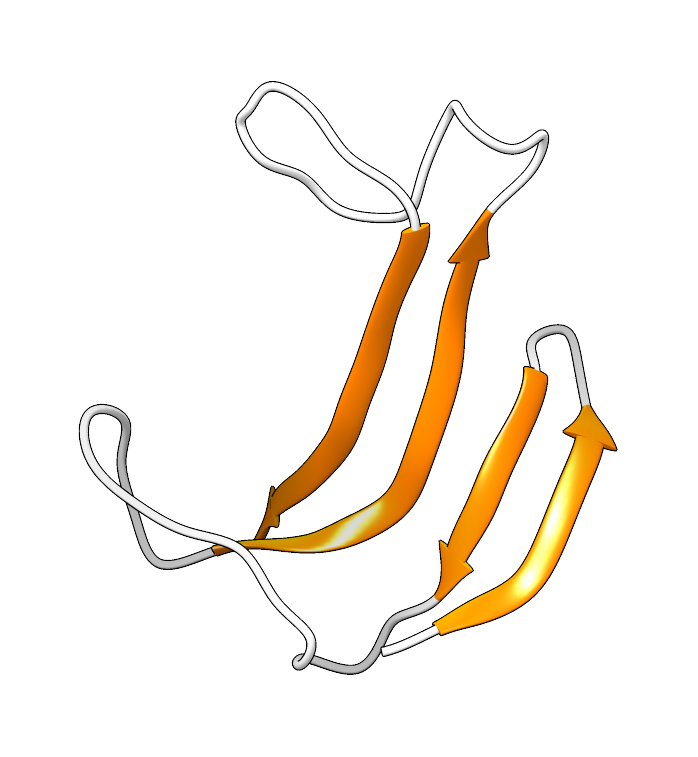
\includegraphics[width=0.4\textwidth]{1ca2_part_betaA_3x3_cropped.png}\label{fig:beta_anti}}
	%\end{center}
	\caption{Example cartoons of parallel and anti-parallel $\beta$-sheets. In parallel $\beta$-sheets, adjacent strands in the sheet are oriented the same way, whereas in anti-parallel $\beta$-sheets, adjacent strands are oriented opposite each other. Created with Chimera~\cite{pettersen2004}.}
	\label{fig:beta}
\end{figure}
Some sections of the polypeptide form neither helices nor sheets, and are called loops.
These sections are more flexible than helices or sheets due the lack of hydrogen bonds, and therefore are useful in connecting the end of one helix/sheet to the beginning of another.
Figure \ref{fig:5nji_ss} shows a cartoon depiction of part of a protein, with different secondary structural elements highlighted in different colors.
	
\begin{figure}
	\centering
	%\begin{center}
	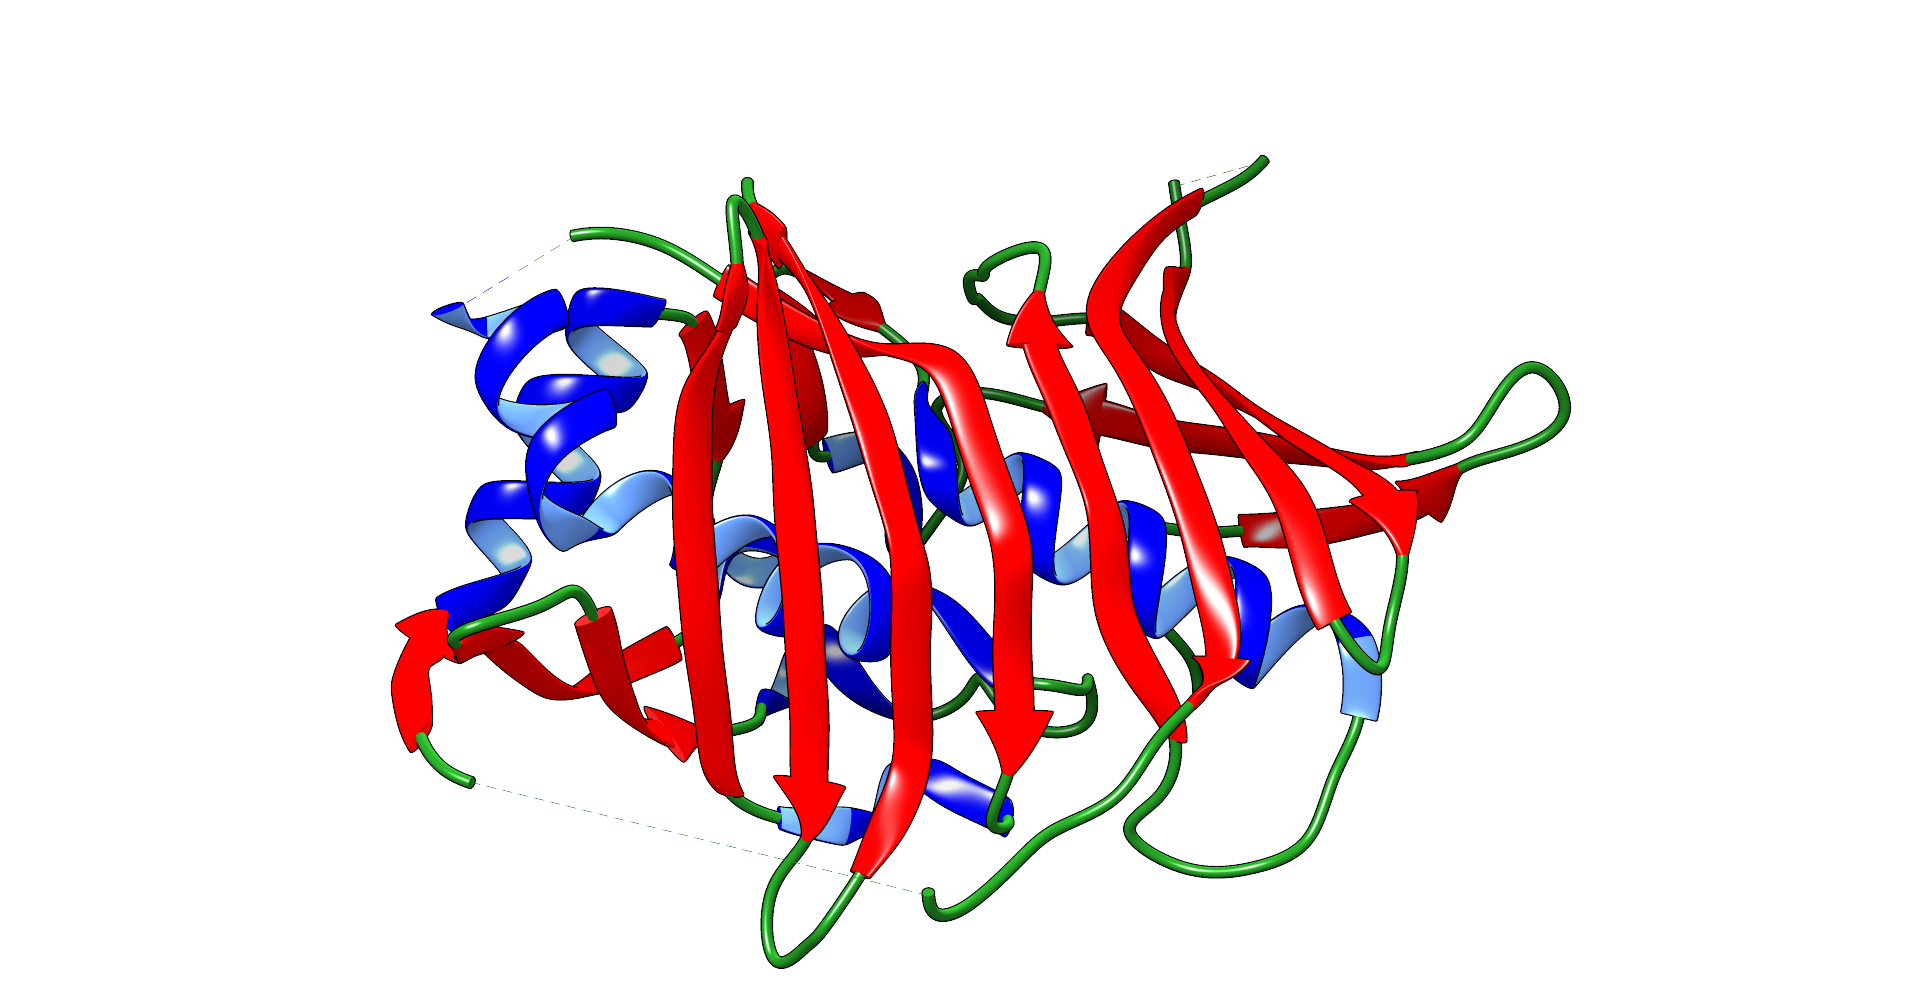
\includegraphics[width=0.8\textwidth]{5nji_ss_ch_3x3.png}
	%\end{center}
	\caption{3D cartoon of the the dehydratase domain of PpsC protein from Mycobacterium tuberculosis (pdb entry 5NJI) showing $\alpha$-helices in blue, $\beta$-sheets in red, and loops in green. Created with Chimera~\cite{pettersen2004}.}
	\label{fig:5nji_ss}
\end{figure}

Helices and sheets provide some rigidity to a polypeptide, but it typically further folds into a 3D structure.
This resulting 3D global structure is called \textit{tertiary structure}.
After folding, some amino acids reside on the surface of a protein while others are buried in the core.
Because water makes up the majority of cellular cytoplasm, protein surfaces have a higher percentage of hydrophilic residues than cores, and cores likewise have a higher percentage of hydrophobic residues than surfaces. 
Protein cores also show higher evolutionary conservation compared to surfaces~\cite{yan2008}.


Finally, in many cases multiple polypeptides combine together into a complex~\cite{scheeffink2003}.
%complexes may be \textit{obligate}, meaning they persist 
The \textit{quaternary structure} describes the manner in which the individual polypeptides combine together to form the complex.
Proteins complexes can be categorized as either \textit{transient} or \textit{permanent}.
This distinction reflects the difference in binding affinity (strength of attraction) between single proteins in the complex, with permanent complexes having higher and transient complexes having lower affinity.
Complexes can also be categorized as either \textit{obligate} and \textit{non-obligate}.
The constituent proteins of obligate complexes typically exist only in the complex, whereas for a non-obligate complex, each constituent protein exist both in the complex and independently.
Transience usually implies non-obligation and obligation usually implies permanence, so a simpler classification of obligate vs. transient is also appropriate~\cite{jones1996}\cite{perkins2010}.
The temporary nature of transient proteins enables complex networks of interaction which give rise to numerous cellular processes and the regulation thereof, including receptor-ligand interaction and signal transduction~\cite{perkins2010}\cite{ofran2003}.
% example of each: substrate-level phosphorylation, protein hormones, transcription factors, antibodies.


\subsection{Protein Interfaces And Their Prediction}

%TODO: mention ligand and receptor

The locus of a protein-protein interaction is the interface, which is comprised of pairs of residues, one from each interacting protein.
These pairs may form a disulfide bond or salt bridge which help anchor the two proteins together~\cite{yan2008}, but this is not always the case\cite~{ofran2003}.
Residues may not attract each other directly but still be considered part of the interface due to proximity.
This is the case when two hydrophobic residues appear near each other in the interface, which is energetically favorable compared to being exposed to water in the surrounding cytoplasm~\cite{yan2008}\cite{ofran2003}.
In the literature, residues are considered part of the interface if they are in contact with residues on the adjacent protein, which is defined either by a sufficient reduction in accessible surface area (see Appendix \ref{appendix:features}), or if the distance between any atom in the residue in question and any atom in the opposing protein is below a threshold~\cite{yan2008}\cite{jones1996}.
This thesis uses the second definition with a threshold of 6 $\AA$, as is common in prior work~\cite{ofran2003}\cite{yan2008}\cite{minhas2014}.

A survey of known protein complex structures from the Research Collaboratory for Structural Bioinformatics (RCSB) Protein Data Bank (PDB) has shown that interfaces have a higher prevalence of hydrophobic residues, lower prevalence of hydrophilic residues, and more evolutionary conservation compared to non-interface surface regions of proteins~\cite{yan2008}.
The higher overall hydrophobicity of an interface leads to energetically favorable states where the interface is able to exclude water by binding to another protein, and the higher degree of conservation shows the functional significance of the interfaces, although conservation is somewhat lower for transient compared to obligate complexes~\cite{jones1996}.
Transient complexes also have a comparatively~\textit{lower} hydrophobicity compared obligate complexes, consistent with the fact that proteins in transient complexes exist outside of the complex, with interfaces exposed to water~\cite{jones1996}.
To overcome the disfavorable energetic effects of burying more hydrophilic residues in an interface, transient interfaces also have relatively higher numbers of hydrogen bonds~\cite{jones1996}.
It has also been shown that transient complexes have less shape complementarity between the participating proteins compared to obligate complexes~\cite{jones1996}.
Lastly, transient interfaces also tend to either be smaller in size(for weakly interacting complexes)~\cite{jones1996}\cite{perkins2010}, or undergo more conformational change when forming(for strongly interacting complexes)~\cite{perkins2010} compared to obligate complexes.
These differences make transient complexes more difficult to distinguish from non-interface surface residues, which is unfortunate given their significant role in cellular processes~\cite{perkins2010}.

Historically, the problem of interface prediction has been formulated in two ways: \textit{partner independent} and \textit{partner specific} prediction.
The former variant considers a single residue from a protein and attempts to answer the question: does this residue form a part of the interface with some other partner protein?
The latter variant considers pairs of residues, each from a different protein, and attempts to answer a more specific question: does this \textit{pair} of residues constitute part of the interface between the two proteins?
The pairwise nature of partner specific prediction allows the consideration of the compatibility of a pair of residues, which has been found to increase performance~\cite{ahmad2011}\cite{minhas2014}.
Methods of interface prediction include \textit{docking methods}, \textit{template-based methods}, and \textit{machine learning methods}.

Docking methods predict the 3D bound formation of two proteins in a complex, from which the interface can be extracted. 
These methods use energy minimization techniques which account for shape complementarity~\cite{chen2003}\cite{zundert2016}.
Unlike template and machine learning methods, docking methods do not require a library of known interfaces in order to make predictions, but are historically poor at accounting for conformational change~\cite{ezkurdia2009}.

Template based methods make predictions based on similarity to a known template protein complex.
The protein of interest is compared to a library of interfaces, and the interface is predicted from similar interfaces.
Template methods rely on a non-redundant template set of protein interfaces and compare entire interfaces to the templates~\cite{tuncbag2011}.

Machine learning methods attempt to directly predict the interface rather than comparing against a template complex or predicting the bound formation, however they still use information from a library of complexes whose interfaces are known.
Machine learning approaches have included use of a neural network~\cite{ahmad2011} and a support vector machine~\cite{minhas2014}.
The latest SVM based approach, PArtner-specific Interacting Residue PREDictor (PAIRpred), uses pairwise kernels which operate on pairs of residues and incorporates both sequence and structural information of residues.
The method performs well compared to existing docking and machine learning methods~\cite{minhas2014}.

The work described in this thesis performs partner specific interface prediction using a more complex data representation and neural network than previous methods.




